\section{Realization}
\label{sec:realization}
%Focus generale sulle tecnologie utilizzate
In this section, we outline the technical aspects concerning the realization of our approach. Therefore we first present the enabler technologies through which we instantiate the design principles presented in \cref{sec:design}. After that, we discuss the interaction workflow between the instantiated technologies. Finally, we show the implementation details.

\subsection{Deployment}
As follows, we bridge the gap between high-level system architecture and its practical realization. \cref{fig:deployment_diagram} depicts a \textit{UML deployment diagram} \cite{koch2002expressive} that aims to help with understanding the instantiated infrastructure. 

%The \texttt{Organization Machine} represents the physical computation \textit{device} embracing the software and hardware entities of the company. The \texttt{Log Recorder}, the \texttt{Log Provider}, and \texttt{Secure Miner} are included in the \texttt{Organization Machine} as abstract \textit{components}. These logical elements incorporate the core functionalities already discussed in \cref{sec:design}. The \texttt{Organization Machine} is characterized by two \textit{execution environment}s, namely the \texttt{Operative System} and the \texttt{TEE}.
In our solution, we make a differentiation between the computational \textit{devices} designated for mining, denoted as \Compo{Miner Machine}s, and those specifically associated with provisioners, identified as \Compo{Provisioner Machine}s. To enhance clarity, we maintain the separation of these devices in the accompanying diagram. However, organizations have the flexibility to opt for integrated technologies that incorporate both mining and provisioning functionalities. %The \Compo{Miner Machine} encompasses the \Compo{Secure Miner} as an abstract component, incorporating its core functionalities, which we presented in detail in \cref{sec:design}. Similarly, the \Compo{Provisioner Machine} includes both the \Compo{Log Recorder} and the \Compo{Log Provider} as abstract components.
We included the \texttt{Log Recorder}, the \texttt{Log Provider}, and \texttt{Secure Miner} (already discussed in \cref{sec:design}) as abstract \textit{components} of the diagram, whose manifestation are described as follow. 

%\Compo{Provisioner Machine}s encompasses \Compo{Log Recorder}s and \Compo{Log Provider}s (already introduced in \cref{sec:design}) as abstract components, incorporating their core functionalities aimed at generating and transmitting event logs. We manifest the \texttt{Log Recorder} in the Process Aware Information System (\Compo{PAIS}) of the organization. These systems help users to handle business processes, including accounting and resource management \cite{Dumas.etal/2018:FundamentalsofBPM}. In our solution, the \texttt{PAIS} provides the \texttt{Log Server} access to event logs. \texttt{Log Servers} implements the functionalities of the \Compo{Log Provider} throigh web services that process remote data request and provides event log to miners. We build \Compo{Log Server}s upon existing web standards such as HTTP\footnote{\url{https://www.w3.org/Protocols/rfc2616/rfc2616.html}. Accessed: \today.}, FTP\footnote{\url{https://www.w3.org/Protocols/rfc959/}. Accessed: \today.}, and Goopher\footnote{\url{https://datatracker.ietf.org/doc/html/rfc1436}. Accessed: \today.}. \Compo{PAIS} and \Compo{Log Server} run on top of the \Compo{Operating System} of the \Compo{Provisioner Machine}.


\Compo{Provisioner Machine}s encompasses \Compo{Log Recorder}s and \Compo{Log Provider}s incorporating their core functionalities aimed at generating and transmitting event logs. Within the organizational context, we manifest the \Compo{Log Recorder} in the Process Aware Information System (\Compo{PAIS}), which plays a crucial role in managing various business processes, including accounting and resource management \cite{Dumas.etal/2018:FundamentalsofBPM}. 
\begin{figure}[t]
	\centering
	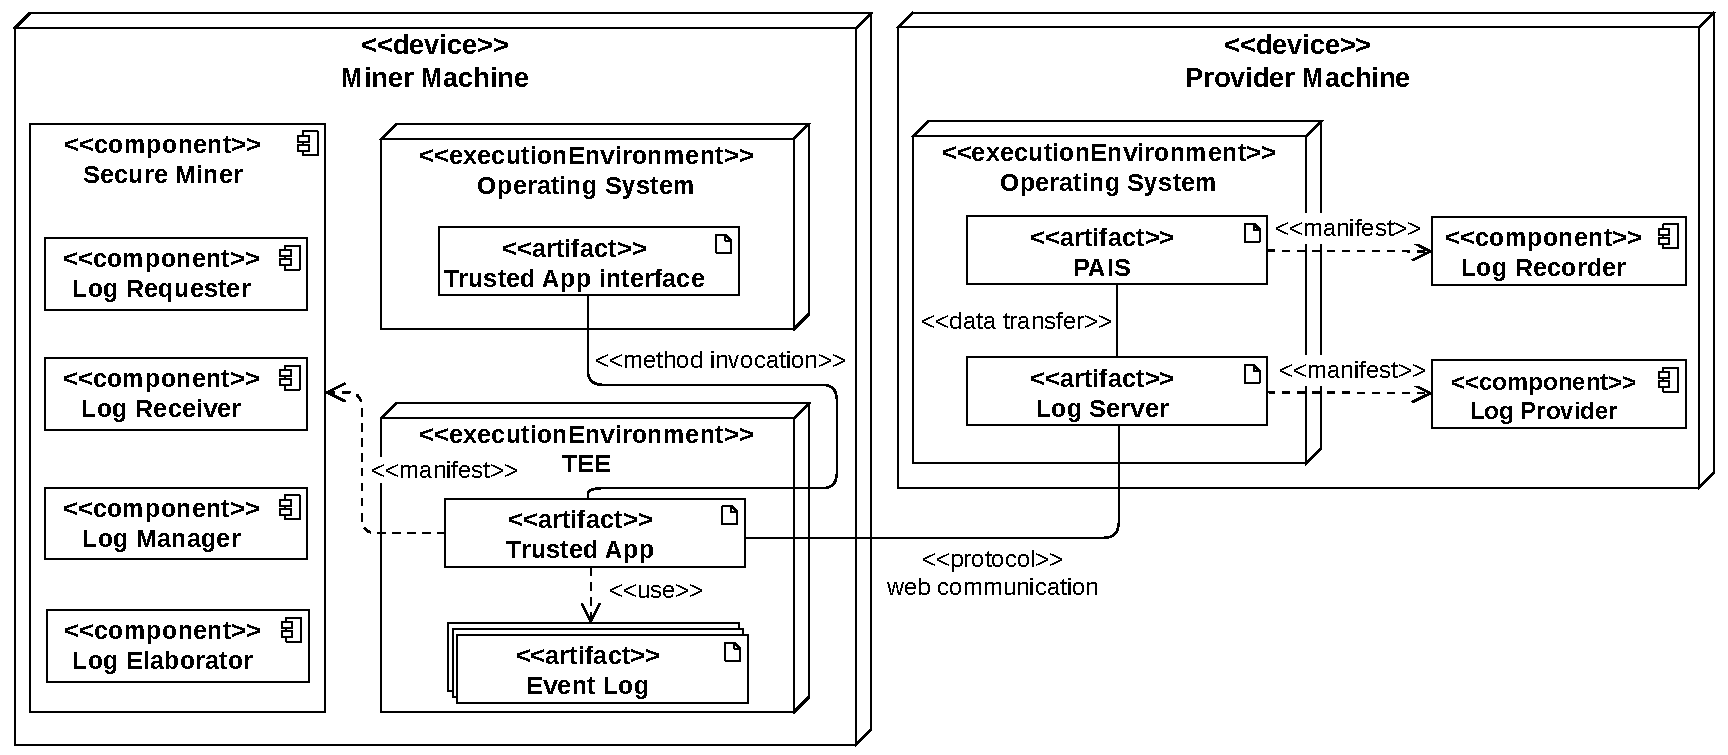
\includegraphics[width=1\linewidth]{content/figures/deploymentdiagram3.pdf}
	\caption{UML deployment diagram.}
	\label{fig:deployment_diagram}
\end{figure}
In our solution, the \Compo{PAIS} grants access to the \Compo{Log Server}, enabling it to retrieve event logs. The \Compo{Log Server}, on the other hand, embody the functionalities of the \Compo{Log Provider}, implementing web services amied at handling remote data requests and providing event logs to miners. \Compo{Log Servers} adheres to established web standards such as HTTP\footnote{\url{https://www.w3.org/Protocols/rfc2616/rfc2616.html}}, FTP\footnote{\url{https://www.w3.org/Protocols/rfc959/}}, and Goopher\footnote{\url{https://datatracker.ietf.org/doc/html/rfc1436}}. Both the \Compo{PAIS} and \Compo{Log Server} run on the top the \Compo{Operating System} of the \Compo{Provisioner Machine}.



%The \Compo{Miner Machine} is characterized by two \textit{execution environment}s, namely the \Compo{Operative System} and the \Compo{TEE}. \Compo{TEE}s create a separated context from the normal \Compo{Operating System} to protect code and data through an hardware-based encryption mechanism. \Compo{TEE}s relies on specific functionalities of the \Compo{Miner Machine}'s CPU that is capable of manage encrypted data in a reserved zone of the RAM\cite{citeTEEhere}. We leverage the security guarantees offered by these technologies to isolate a  \Compo{Trusted App} that fulfills the functionalities of the \Compo{Secure Miner} and its subcomponents. The \Compo{Trusted App} collects the logic to generate verifiable data requests, receive external event logs, store them in the \Compo{TEE}, and apply process mining algorithms. Procedures executed by the \Compo{Trusted App} are tamperproof. The \Compo{TEE} ensures that the code of the \Compo{Trusted App} executed within it is protected from malicious manipulations and unauthorized access from entities running inside the \Compo{Operating System}. Furthermore, we employ the isolated environment of \Compo{TEE} to store \Compo{Event Log}s of provisioner organizations inside the \Compo{Miner Machine}. The \texttt{TEE} provides a mechanism to protect this sensitive information without exposing it to the \Compo{Operative System}. The \Compo{Trusted App} is the only entity that can access the \Compo{Event Log}s, and feed them to process mining algorithms. Users can communicate with the \Compo{Trusted App} via the \Compo{Trusted App Interface}. The \Compo{Trusted Application} offers secure methods to safely receive information from the \Compo{Operative System} and outsource the outputs of the computation. These methods are invoked by the \Compo{Trusted App Interface} instantiating the only communication channel with the \texttt{Trusted App}.

The \Compo{Miner Machine} is characterized by two distinct \textit{execution environments}: the \Compo{Operating System} and the Trusted Execution Environment (\Compo{TEE}). \Compo{TEE}s establish an isolated context separate from the normal \Compo{Operating System}, safeguarding code and data through hardware-based encryption mechanisms. This technology relies on specialized components of the \Compo{Miner Machine}'s CPU capable of managing encrypted data within a reserved section of RAM \cite{TEEHERE}. We leverage the security guarantees provided by \Compo{TEE}s to isolate a \Compo{Trusted App} responsible for fulfilling the functions of the \Compo{ Secure Miner} and its associated subcomponents. The \Compo{Trusted App} consolidates the logic required for generating verifiable data requests, receiving external event logs, securely storing them within the \Compo{TEE}, and executing process mining algorithms. All procedures executed by the \Compo{Trusted App} are tamper-proof. The \Compo{TEE} ensures the integrity of the \Compo{Trusted App} code, protecting it against malicious manipulations and unauthorized access by entities operating within the \Compo{Operating System}. Additionally, we utilize the isolated environment of the \Compo{TEE} to securely store event logs from provisioner organizations within the \Compo{ Miner Machine}. The \Compo{TEE} safeguards this sensitive information alongside a unique asymetric key couple used for attestation purposes (i.e., public and private keys), preventing exposure to the \Compo{Operating System}. Access to data located in the \Compo{TEE} is restricted solely to the \Compo{Trusted App}. Users interact with the \Compo{Trusted App} through the \Compo{Trusted App Interface}, which serves as the exclusive communication channel. The \Compo{Trusted App} offers secure methods, invoked by the \Compo{Trusted App Interface}, for safely receiving information from the \Compo{Operating System} and outsourcing the results of computations, maintaining a high level of data security.

The interaction between the newly introduced technologies is elucidated as follows.
\begin{comment}
\begin{figure}[t]
\centering
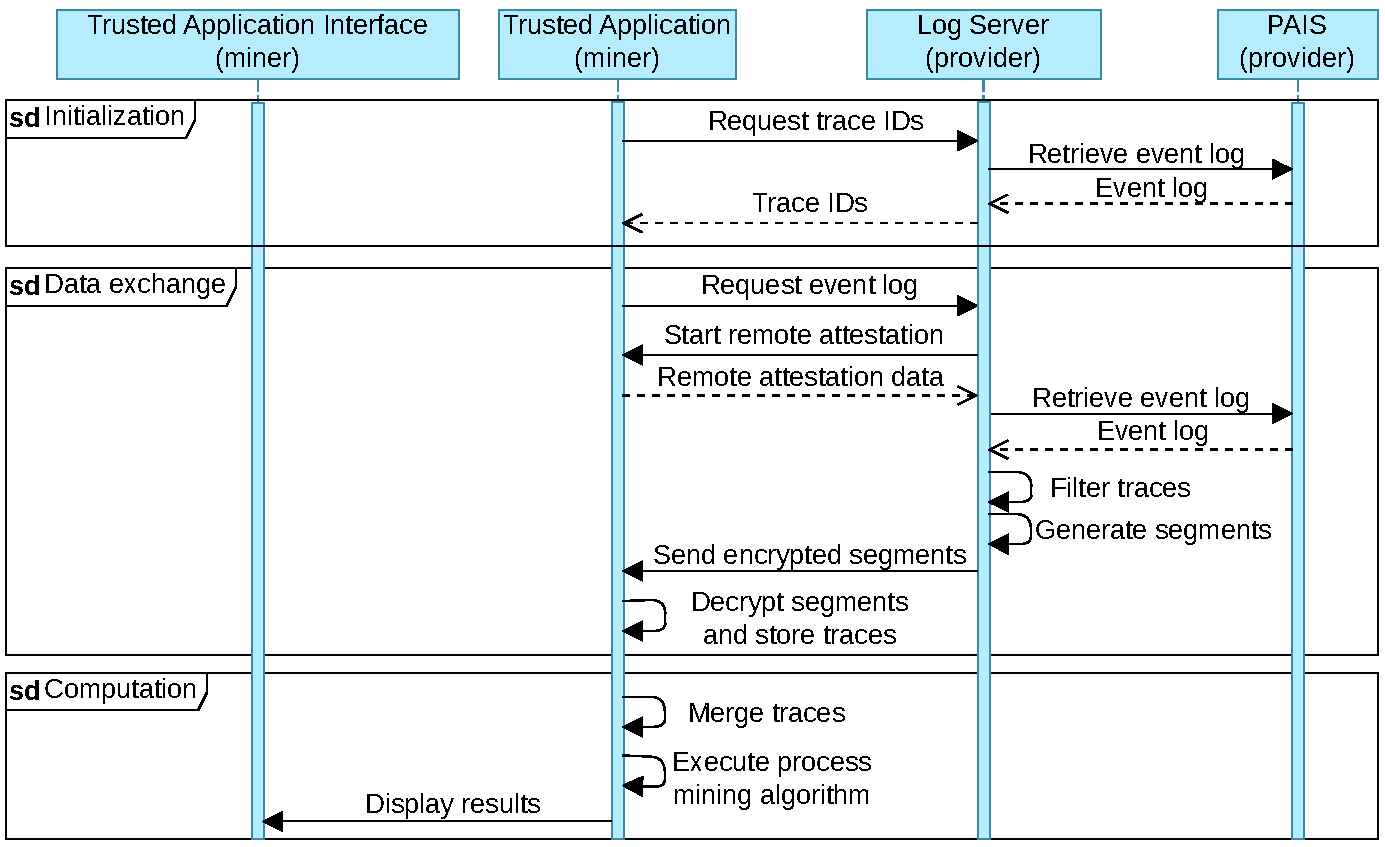
\includegraphics[width=0.9\linewidth]{content/figures/sequencediagram.pdf}
\caption{UML sequence diagram.}
\label{fig:sequence_diagram}
\end{figure}
\end{comment}
%orizontale

    \begin{figure}[t]
     \subfloat[][Initialization]{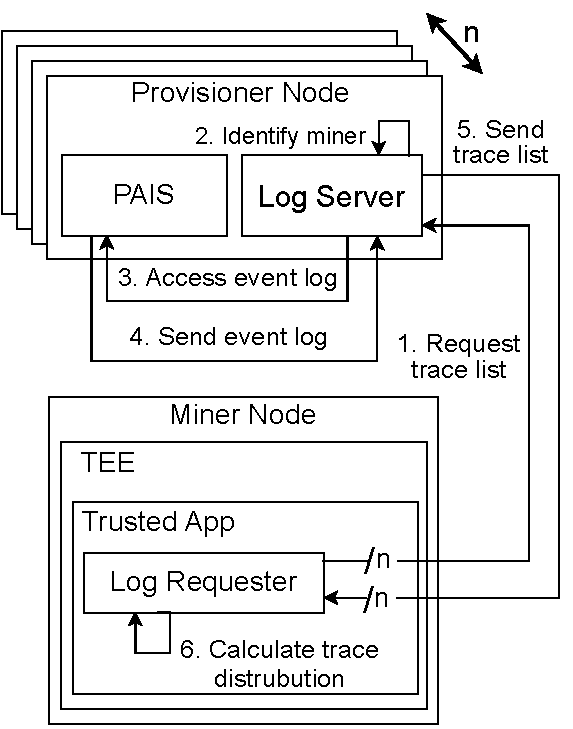
\includegraphics[width=0.29\linewidth]{content/figures/initializationworkflow.pdf}}\label{<figure1>}\hfill
     \subfloat[][Remote Attestation]{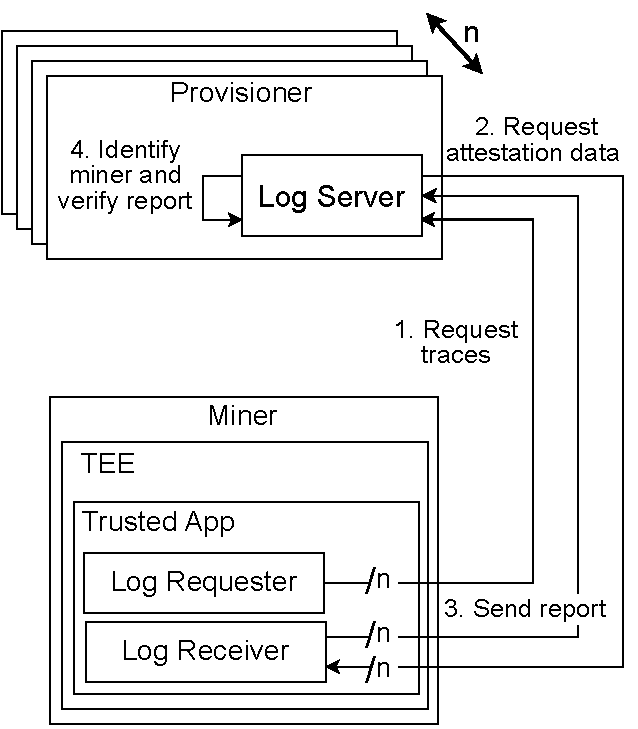
\includegraphics[width=0.32\linewidth]{content/figures/attestationworkflow.pdf}}\label{<figure1>}\hfill
     \subfloat[][Data Transmission]{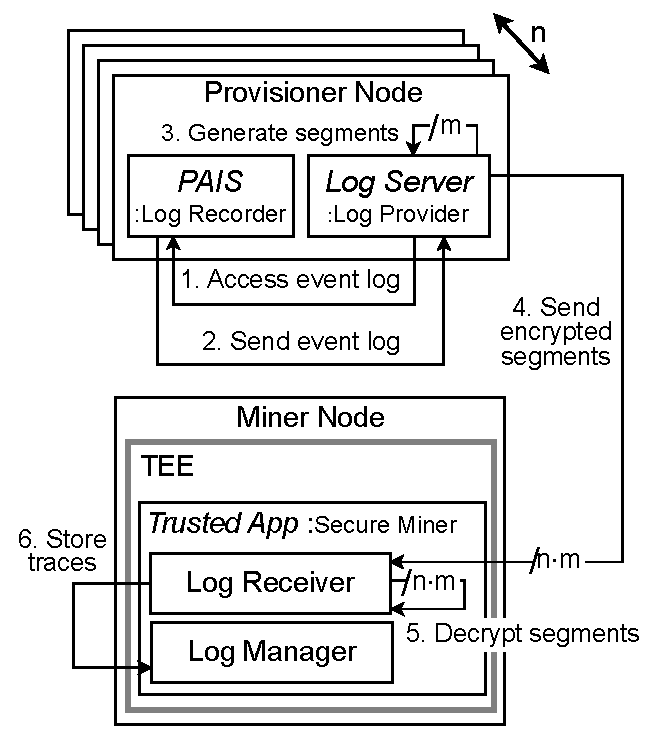
\includegraphics[width=0.33\linewidth]{content/figures/datatransmissionworkflow.pdf}}\label{<figure1>}\hfill
%     \subfloat[][Computation]{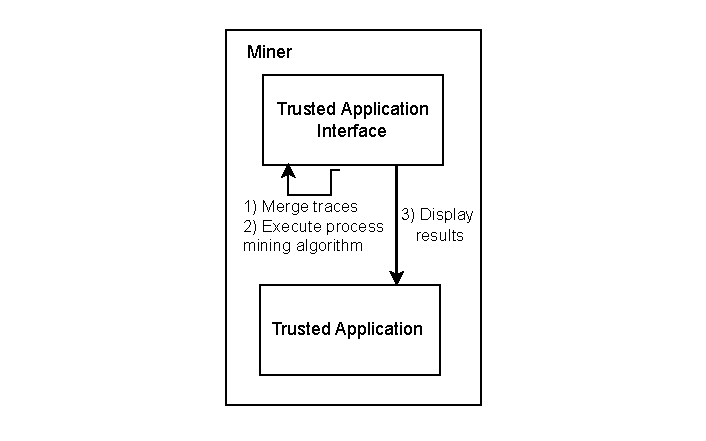
\includegraphics[width=0.32\linewidth]{content/figures/flow_computation.pdf}}\label{<figure1>}
     \caption{Schematization of the initialization, remote attestation and data transmission phase.}
     \label{flow}
    \end{figure}


\subsection{Workflow}
%

%
We separate the workflow into subsequent processes, namely \textit{initialization},\textit{remote attestation}, \textit{data transmission}, and \textit{computation}.
The parties involved in the workflow are a miner (i.e., an organization that executes process mining algorithms) and one or more providers (i.e., partner organizations that serve their event logs). %We distinguish three different phases of the process namely the \textit{initialization}, the \textit{data exchange}, and the \textit{computation}.
%\todo{CDC: We need an example. We must provide an example of (simplified) event log excerpt, with a few traces taken from the scenario, show which bits reside in the different machines, and show the final merged event log. Then, discuss it during the description of the workflow, showing how we get from the original pieces to the final one. This description takes time.}

\textbf{Initialization.} In the initialization, the miner's \texttt{Trusted Application} requests preliminary information from the providers' \texttt{Log Server} concerning the event logs of an inter-organizational business process. After authenticating the sender, the involved \texttt{Log Server}s retrieve the local event log from the \texttt{PAIS} and respond to the miner by providing the list of trace IDs in the event log. Hence, the \texttt{Trusted Application} collects the responses and stores them in the \texttt{TEE}.

\textbf{Remote Attestation.} \todo[inline]{Talk specifically of remote attestation}

\textbf{Data Transmission.} Once recorded the preliminary information, the miner starts the data exchange. Therefore, its \texttt{Trusted Application} sends data requests to the \texttt{Log Servers}. The requests include as parameters the list of trace ids and the segment size. Subsequently, the \texttt{Log Server}s starts the \textit{remote attestation} procedure, thanks to which they can verify that the sender of the log request: is a \texttt{Trusted Application} running inside a \texttt{TEE}; comes from a partner organization. This operation involves the exchange of additional messages between the \texttt{Log Server} and the \texttt{Trusted Application}. If the procedure is successful, the miner's identity is verified.
Subsequently, the \texttt{Log Servers} retrieve the local event log and filter its traces according to the trace IDs sent by the \texttt{Trusted Application}. Filtered event logs are split into several segments containing traces whose dimension does not exceed the segment size parameter. \texttt{Log Servers} encrypts the segments and send each of them to the \texttt{Trusted Application}. The \texttt{Trusted Application} decrypts the received segments, extracts the traces, and stores them in \texttt{Event Log}s inside the \texttt{TEE}.

\begin{wrapfigure}[9]{r}{0.33\textwidth}
   \vspace{-2em}
  \centering
  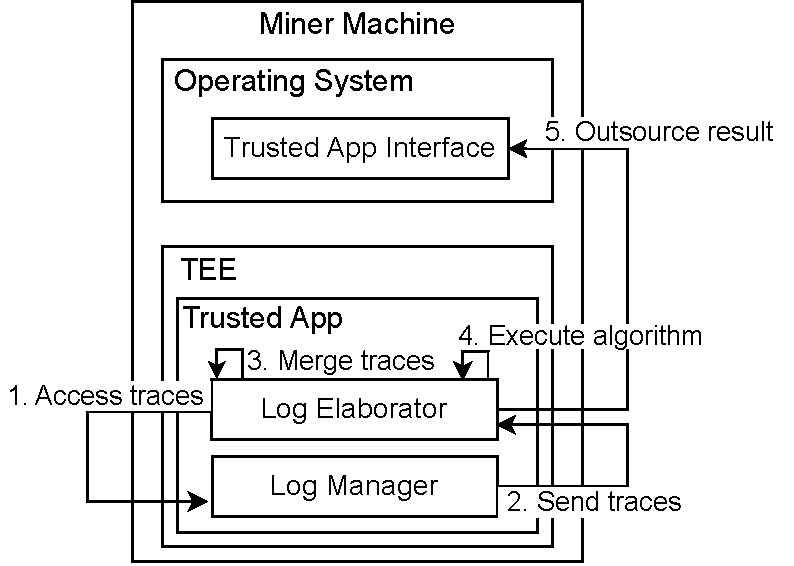
\includegraphics[width=1\textwidth]{content/figures/computationworkflow.pdf}
  \caption[A gull]{Schematization of the computation phase.}
  \vspace{-6pt}
\end{wrapfigure}
\textbf{Computation.} To start a computation routine, the \texttt{Trusted Application} needs all partner organizations to have delivered traces having the same ID. When this occurs, the \texttt{Trusted Application} merges external traces with the owned one. Assembled traces are used as parameters of process mining algorithms executed by the \texttt{Trusted Application} that presents the computation results to the users via the \texttt{Trusted Application Interface}.







\subsection{Implementation}
\label{sec:implementation:details}
In this section, we expound the implementation of our paper. The proposed implementation integrates a trusted application within a secure execution environment, complemented by the inclusion of event logs to address the issue outlined in the motivating scenario. The source code is accessible at the following URL: \url{https://github.com/dave0909/TEExProcessMining/}.


To realize the implementation of trusted applications, we employed EGo,\footnote{https://www.edgeless.systems/products/ego/} a framework designed for encoding trusted application in the Go\footnote{https://go.dev} programming language. Contained within the trusted application is the \Compo{Secure Miner} module, which facilitates the requisition, administration, and processing of logs from external organizations. To exemplify our approach's capability for conducting process analysis, we implemented a renowned process discovery algorithm within the \Compo{Secure Miner}. 










\begin{comment}
In this section, we describe the implementation of our paper. The implementation proposed integrates a trusted application running in a trusted execution environment and some event logs generated to address the solution proposed in the motivating scenario. The code is available at the following address: \url{https://github.com/dave0909/TEExProcessMining/}

We have encoded a well-known process discovery algorithm within the \texttt{Secure Miner} component to demonstrate the capability of conducting process analytics tasks with our approach.
To implement the trusted applications, we used the EGo,%
\footnote{https://www.edgeless.systems/products/ego/} 
a framework to encode programs for TEEs in %. EGo makes it possible to develop trusted applications programmed in 
GO.%
\footnote{https://go.dev}
% We developed the Trusted Application (TA) within the TEE with the same language. 
Within the TA there is the ``Secure Miner" module, which allows logs from other organizations to be requested, managed, and processed. Log processing is made possible by the implementation of the ``Heuristc Miner" process mining algorithm\ref{weijters2006process}, which takes the log traces as input and performs a discovery operation.
The output of the algorithm is a PNML\footnote{https://www.pnml.org}(Petri Net Markup Language) which allows the representation of Petri nets that graphically illustrate the model calculated by the algorithm. 
%The output of the algorithm is a file with the extension '.pnml'. PNML\footnote{https://www.pnml.org}(Petri Net Markup Language) is a markup language that allows the representation of Petri nets that graphically illustrate the model calculated by the algorithm. 
In order to generate the graphic image of the Petri net, we used the WoPed\footnote{https://woped.dhbw-karlsruhe.de} software, which takes as input a PNML file and provides the graphic representation of the Petri net. 

%Log provider language
Another fundamental module within the TA is the Log Provider. We wrote this part of TA in Go. The log provider is listening for log requests from other organizations on one of the ports set by the owning organization. When an organization decides to start the mining process, it requests the logs of the other organizations. The log providers accepts requests made by the organization that starting the mining operation and forwards its log.
\end{comment}
